\section{O \textit{middleware} uOS}
\label{sec:uos}
	 
	O \textit{middleware uOS}, projeto do grupo de pesquisa \textit{UnBiquitous} da Universidade de
	Brasília, tem como objetivo a integração das aplicações no ambiente inteligente e foca na
	adaptabilidade dos serviços presentes nos mais diversos dispositivos. Desta forma, os serviços
	passam a ser compartilhados de uma forma menos intrusiva \cite{buzeto}. Conforme apresentado na
	figura~\ref{fig:dsoa}, o \textit{middleware uOS} atua como uma camada entre as aplicações
	e~\textit{drivers}.
	
	\begin{figure}[htb]
		\centering 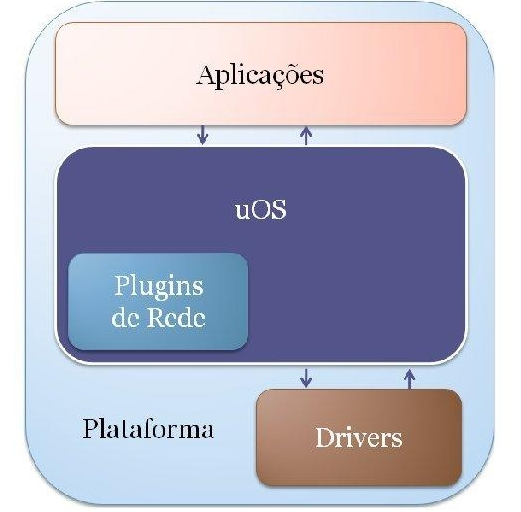
\includegraphics[scale=.35]{figuras/cap2/dsoa.jpg}
		\caption{\textit{Middleware uOS~\cite{buzeto}.}}
		\label{fig:dsoa} 
	\end{figure}
	 
	O \textit{uOS} segue os conceitos propostos pela ~\textit{DSOA} (\textit{Device Service Oriented
	Architecture}) para modelagem do ambiente inteligente. Nessa arquitetura são definidos o modelo
	de comunicação a ser utilizado, implementando algumas características definidas pelo
	~\textit{SOA (Service Oriented Architecture)}~\cite{buzeto_11}. Por causa da diversidade e capacidade de
	processamento dos diversos dispositivos presentes no \textit{smart space}, foi criado um conjunto
	de protocolos para a computação ubíqua, implementada sobre o ~\textit{middleware uOS}, denominada de ~\textit{uP
 	(Ubiquitous Protocols)}, viabilizando uma maneira simplificada e padronizada para a troca de
 	informações entre esses dispositivos. O \textit{uP} permite uma interação entre os dispositivos,
 	levando-se em consideração a heterogeneidade das plataformas, os diferentes modelos de comunicação
 	e interação com o ambiente. Desta forma, o \textit{uP} possibilita a descoberta de novos
 	dispositivos no ambiente e a representação dos recursos através de \textit{drivers}.
	
	O \textit{uOS} foi desenvolvido na linguagem JAVA, possibilitando a utilização do mesmo nos mais
	diversos dispositivos que a ofereçam suporte. Ele se encontra disponível em duas versões: uma
	\textit{mobile}, sob a plataforma JME (\textit{Java Micro Edition}), e uma seguindo a plataforma
	JSE (\textit{Java Standart Edition}). Esta última foi também portada para a utilização em
	dispositivos Android. Viabilizando sua utilização tanto em dispositivos limitados (usando a
	plataforma \textit{mobile} ou Android) à outros mais capazes.
	
